%Grasp
La metaheurística Grasp consiste en generar varias soluciones iniciales a partir de una heurística golosa aleatorizada y correr búsqueda local sobre ellas. La solución final es la mejor encontrada tras todas las búsquedas locales.
Sea $S$ el conjunto de soluciones iniciales, el algoritmo que se usa es el siguiente:\\\\
\hspace*{1 cm} Mientras no se alcance el criterio de terminación:\\
\hspace*{2 cm} Obtener $s \in S$ mediante una heurística golosa aleatorizada.\\
\hspace*{2 cm} Mejorar $s$ mediante búsqueda local.\\
\hspace*{2 cm} Recordar la mejor solución obtenida hasta el momento.\\
%Solucion inicial
\subsubsection{Solución inicial}

Usamos Dijkstra como nuestra heurística golosa, pero modificado para agregarle aleatoriedad. El factor aleatorio consiste en que en cada iteración de Dijkstra, en vez de tomar el nodo no visitado que minimiza la función objetivo, tomamos uno de entre los $beta$\footnote{\label{$beta$}: Luego de experimentar con distintos valores, encontramos que $beta$=10 era un valor que presentaba suficiente aleatoriedad.} menores, al azar.

Dada la aleatoriedad de la solución inicial, es posible que ésta no sea factible. En caso de obtener una solución de ese tipo, no ejecutamos búsqueda local.

Utilizamos Dijkstra con la función de peso $\omega_1$. De esta forma se intenta dar variedad a las soluciones iniciales, pero al mismo tiempo que éstas sean factibles - es decir, que cumplan con la restricción de $\omega_1 < K$ - en su mayoría.

\subsubsection{Criterio de terminación}

Usamos 3 criterios de terminación distintos al mismo tiempo. De alcanzarse alguno de los criterios, se termina la ejecución del algoritmo.

Los criterios que usamos son:
\begin{itemize}
\item Cantidad máxima de iteraciones.
\item Cantidad máxima de iteraciones sin haber encontrado mejoras.
\item Cantidad máxima de iteraciones sin haber encontrado una solución inicial factible.
\end{itemize}

Parametrizamos estos criterios usando $n$. Para elegir valores adecuados realizamos distintas experimentaciones sobre grafos de tipo \textit{mágico} con baja, media y alta densidad. Los resultados obtenidos se pueden ver en los siguientes gráficos:

\begin{figure}[H]
\begin{center}
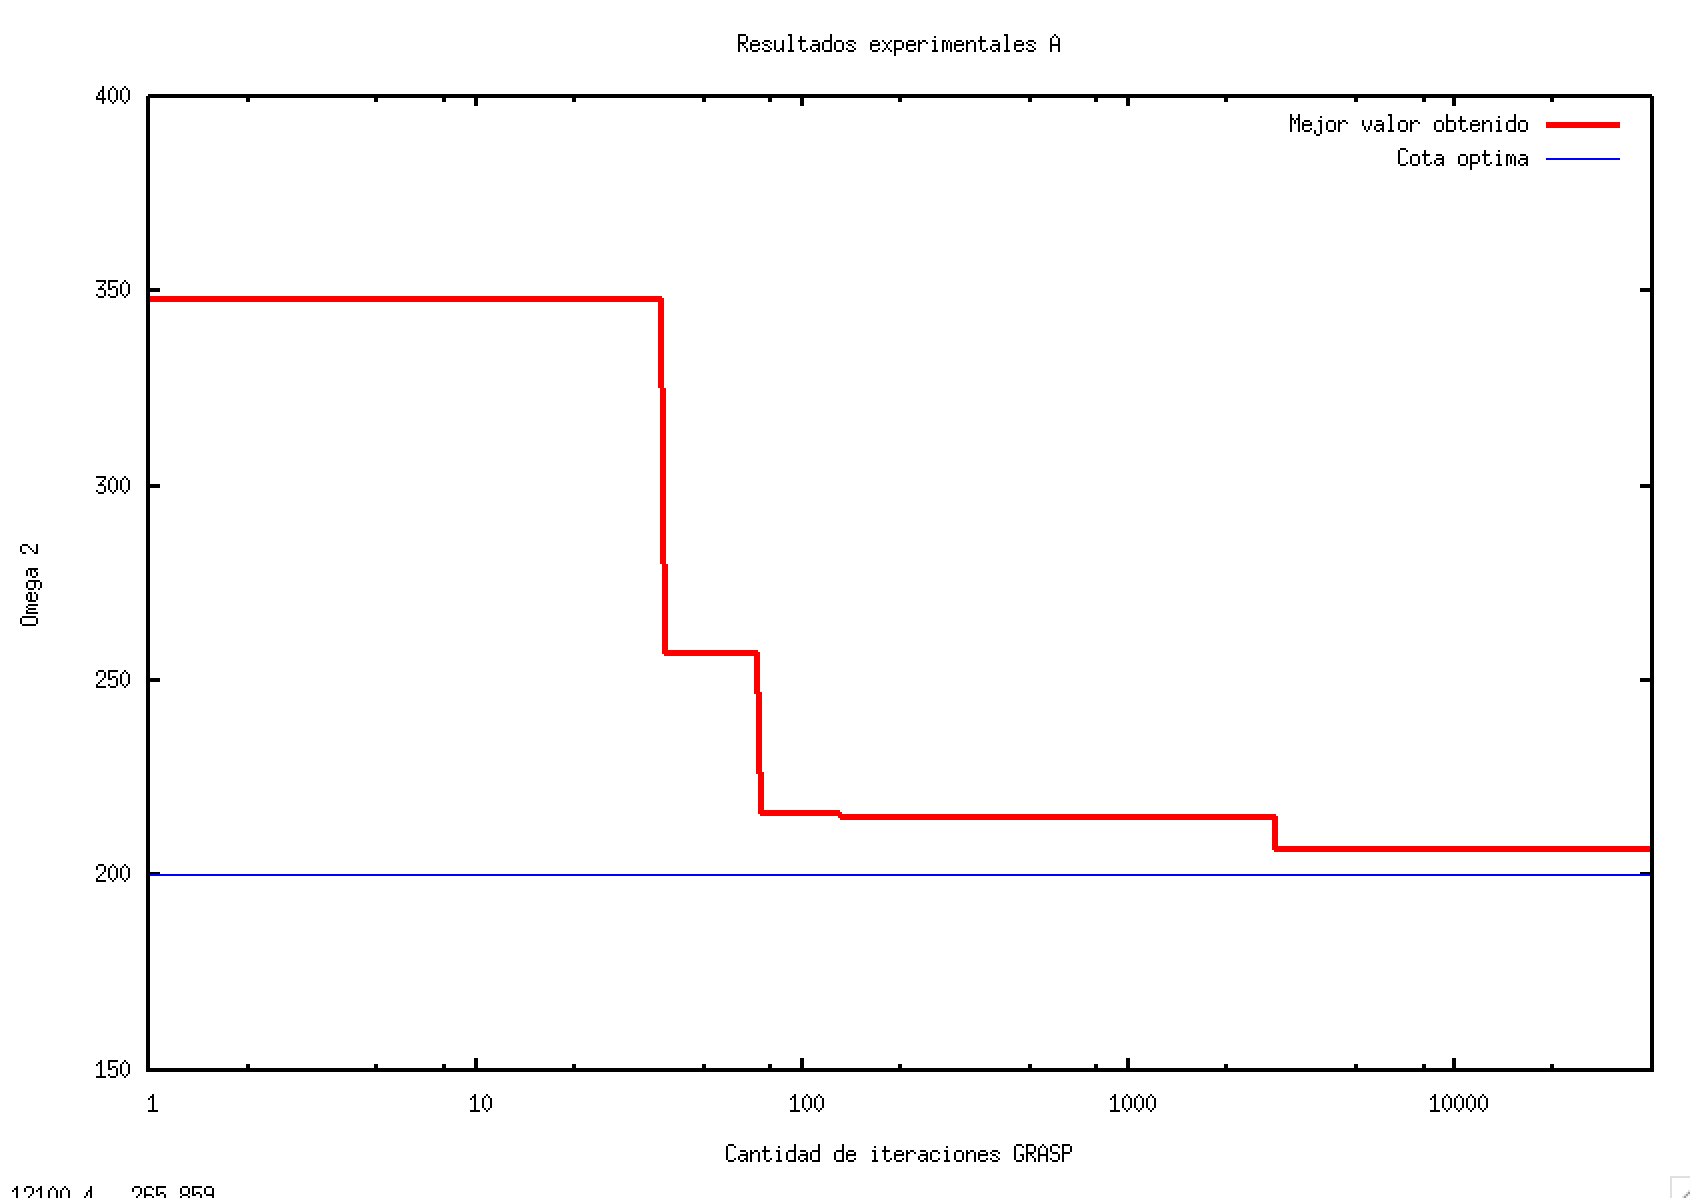
\includegraphics[angle=0, scale=.5]{imagenes/iteraciones-GRASP-A.png}
\label{Resultados experimentales A}
\end{center}
\end{figure}

\begin{figure}[H]
\begin{center}
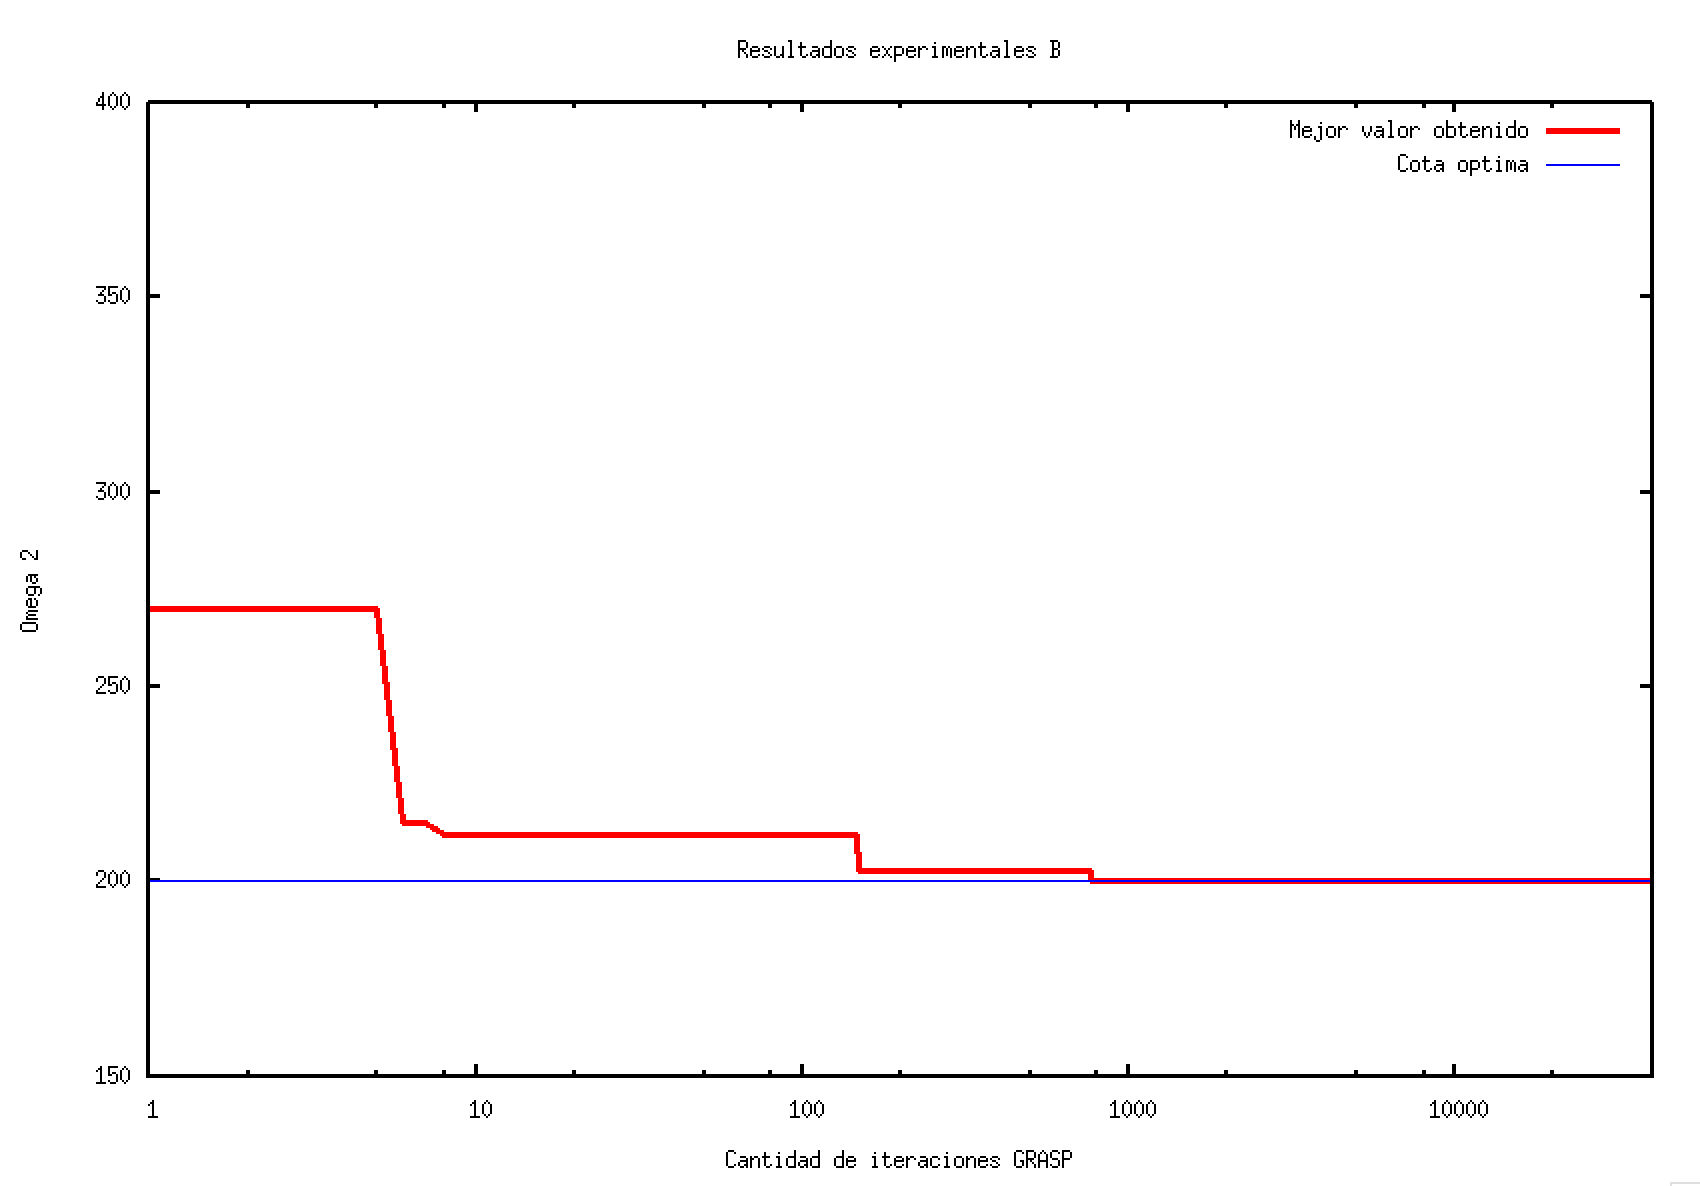
\includegraphics[angle=0, scale=.5]{imagenes/iteraciones-GRASP-B.png}
\label{Resultados experimentales A}
\end{center}
\end{figure}

\begin{figure}[H]
\begin{center}
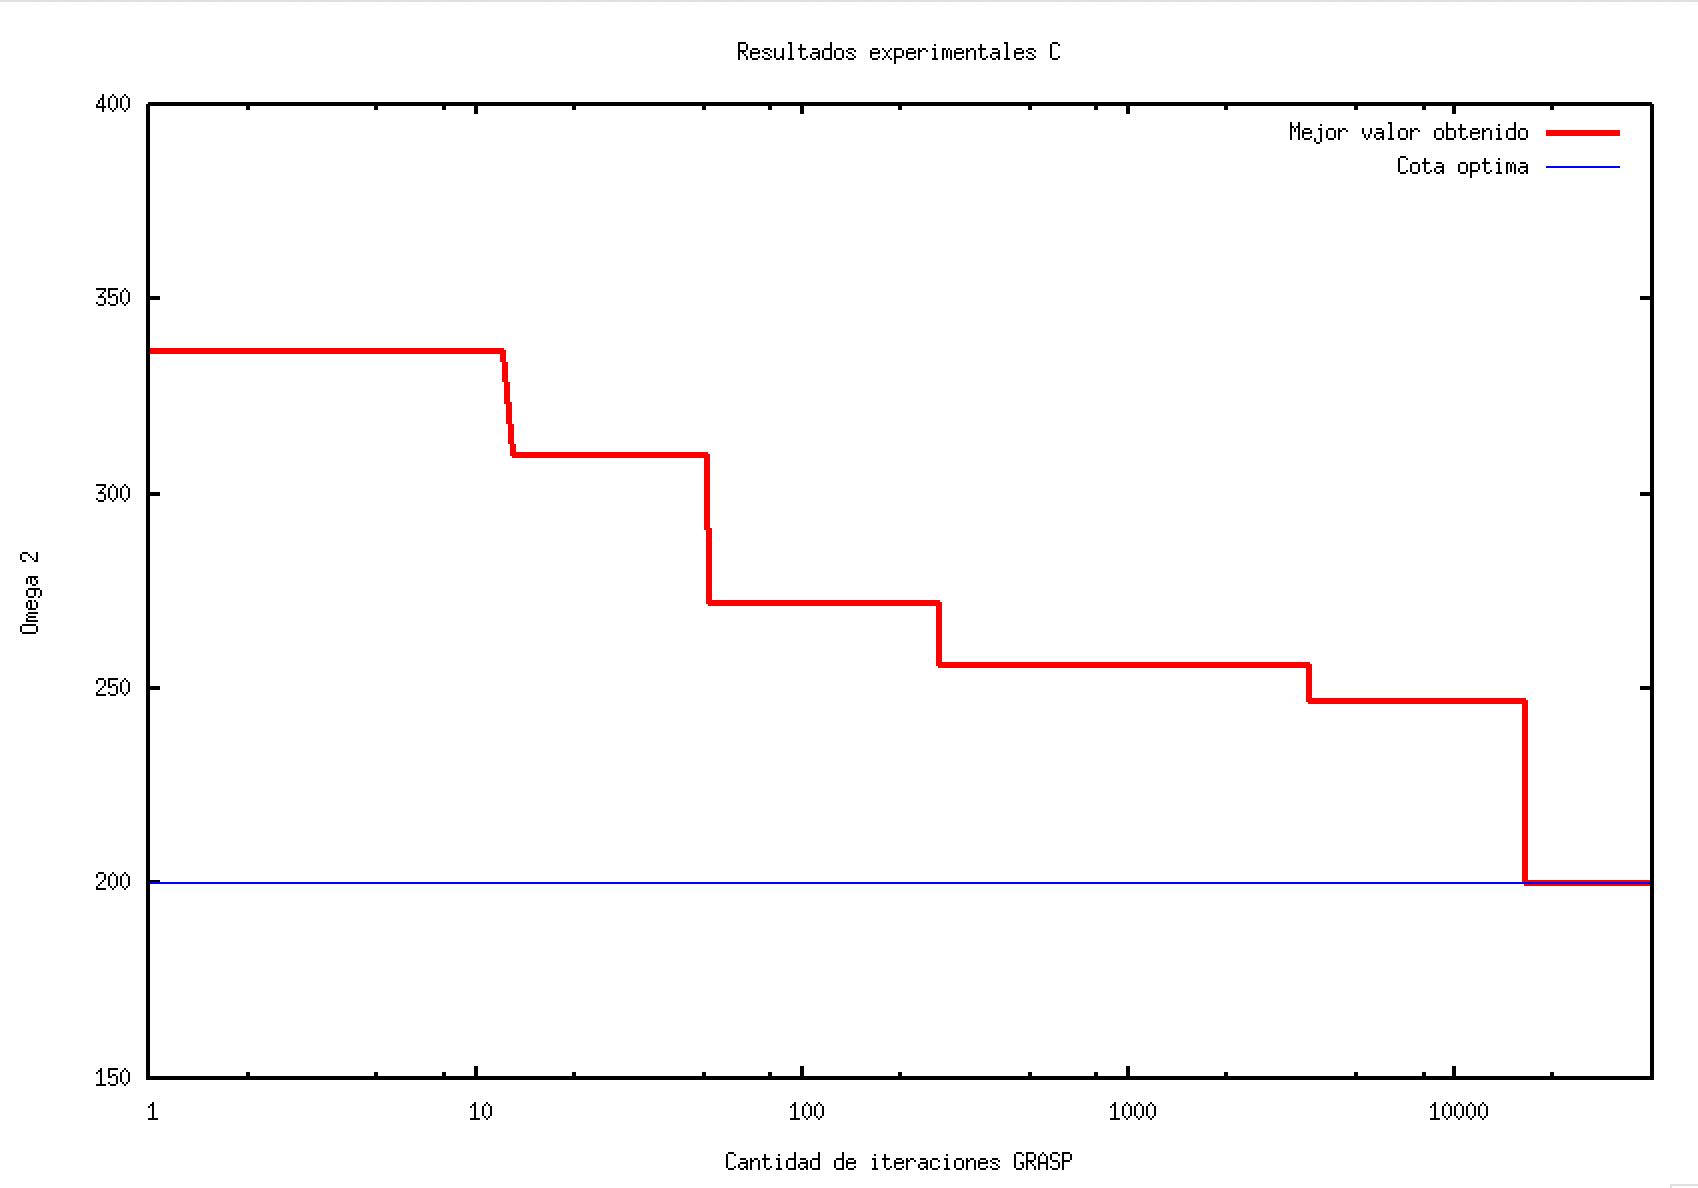
\includegraphics[angle=0, scale=.5]{imagenes/iteraciones-GRASP-C.png}
\label{Resultados experimentales C}
\end{center}
\end{figure}

Las experimentaciones A, B y C se realizaron corriendo GRASP usando grafos de entrada de 200 nodos y 400, 4000 y 10000 ejes respectivamente. Cada una de las experimentaciones ejecuta 40000 iteraciones\footnote{Se consideró que $n^2$ era una cantidad de iteraciones suficientemente grande como para realizar las pruebas. En caso de resultar insuficientes se realizaría una nueva prueba con una cantidad mayor.} en total, realizando en cada una un muestreo del valor de la mejor solución obtenida hasta el momento.

Cada figura muestra como evoluciona el valor de $\omega_2$ a medida que aumentan las iteraciones. Además, fue graficado el camino óptimo, cuya deducción es posible gracias a las características de los grafos utilizados, en donde para el mismo el valor de $\omega_2$ es igual a la cantidad de nodos del grafo, menos uno, es decir 199. De esta forma, pudimos comparar cuán buenos fueron los valores obtenidos.

Luego de tomar las muestras, dada la naturaleza de los datos obtenidos, decidimos utilizar escala logarítmica en el eje X para facilitar la visualización de los resultados, ya que como característica general notamos que se presenta una veloz \textit{mejoría} en las soluciones durante las primeras iteraciones. Esta característica se encuentra fuertemente acentuada en los \textbf{experimentos A y B}, en los que se puede observar que durante las \textbf{primeras 1000 iteraciones}, es decir el primer $2,5\%$ del muestreo total, la \textbf{distancia a la solución óptima} realiza una disminución crítica, de $150$ a $10$ en el caso del \textbf{experimento A}, y de $70$ a $0$ en el caso del \textbf{experimento B}. El \textbf{experimento C}, también demuestra una notable mejoría en la distancia a la solución óptima, de $150$ a $50$, en el transcurso de las primeras 1000 iteraciones; la misma es, sin embargo, mucho más escalonada. La vertiginosa velocidad de acercamiento al valor óptimo (en comparación con la cantidad de iteraciones realizadas) justificó la utilización de esta escala. 

Nuestro objetivo al momento de considerar los valores óptimos para los criterios de parada se basó en encontrar una forma de elegirlos de manera tal que los mismos se adecúen correctamente a grafos de variada densidad. 

Creando grafos con una cantidad fija y representativa de nodos, y variando la densidad de aristas de los mismos, encontramos que para el caso de grafos de 200 vértices, el algoritmo puede iterar aproximadamente 10000 iteraciones \textbf{sin encontrar mejoras}. Este valor lo obtuvimos del anteúltimo salto de la \textbf{experimentación C}, y se corresponde con $n^2 / 4$.

La \textbf{máxima cantidad de iteraciones necesarias} para encontrar un \textbf{valor considerablemente cercano al óptimo} fue observada también en la \textbf{experimentación C}, siendo esta de alrededor de 20000 iteraciones, o $n^2 / 2$.

Para elegir un valor para la \textbf{cantidad máxima de iteraciones que pueden transcurrir sin haber encontrado una solución inicial factible}, tomamos el mismo valor que para la cantidad máxima de iteraciones sin haber encontrado mejoras, es sea $n^2 / 4$. Esto se fundamenta en que si no se encontró una solución inicial factible, tampoco se mejoró la última solución encontrada y por ende este criterio nos sirve para acotar el valor.

Además de encontrar valores que consideramos útiles y adecuados para los ya mencionados criterios, encontramos interesante la influencia de la densidad de los grafos en el comportamiento del algoritmo. Dada una entrada de baja densidad de aristas, es más difícil que el mismo encuentre una buena solución inicial, y más aún \textbf{mejorar una solución relativamente cercana al óptimo} (en el muestreo concreto se puede observar que transcurren unas 39000 iteraciones, las últimas, en donde sólo se sucede una pequeña mejora de la solución). Dedujimos que esto sucede porque en la el grafo A hay pocos caminos (dada la baja densidad) y por consiguiente hay menos chances de encontrar los \textbf{mejores caminos}. Creemos que por esto sucede que no se logra llegar al óptimo aún luego de correr 40000 iteraciones, y por tal motivo creemos que llegado este punto es inútil seguir intentando encontrar un camino mejor.

El experimento que muestra el mejor comportamiento del algoritmo es el B, usando densidad media. Logra encontrar el camino óptimo mucho antes de llegar a nuestra cota para la cantidad de iteraciones: tarda alrededor de 1000 iteraciones (muy por debajo de las 20000($n^2 / 2$) iteraciones que utilizaremos finalmente como cota máxima). Además, logra encontrar un camino inicial bastante mejor que las otras dos opciones($\omega_2$ = 250 frente a $\omega_2$=300+ de A y C, es decir un $25\%$ mejor dado el óptimo de 200). 

Por último, creemos que la experimentación C muestra un caso representativo de la gran filosofía GRASP, ya que se que mejora la solución escalonadamente hasta dar con la óptima, luego de varias mejoras parciales.


\subsubsection{Búsqueda local}

La búsqueda local que realizamos es la misma que en el apartado anterior.

\subsubsection{Pseudocódigo}

El algoritmo está implementado en la función \texttt{main}:

\begin{algorithm}[H]
\caption{$main$(int tipo\_solucionInicial, Graph g, Nodo n1, Nodo n2)}
\begin{algorithmic}[1]
  \State crearMatrizCaminosMinimos(g)
  
  \State int $n = |nodes(g)|$
  \State int iteracionesSinMejorarCount = 0
  \State int iteracionesSinMejorarMax = n
  \State int iteracionesMax = $n \times log(n)$
  \State int iteracionesSinInitialPathCount = 0
  \State int iteracionesSinInitialPathMax = n
  \State mejorSolucion = NULL
  \For{i=0; i$<$iteracionesMax; i++}
  	\State Solution solucion = obtenerSolucionInicial(tipo\_solucionInicial, g, n1, n2)	
	\If{$\omega_1$(solucion) $>$ K}
    		\State iteracionesSinInitialPathCount++
		\If{iteracionesSinInitialPathCount $\geq$ iteracionesSinInitialPathMax}
			break
		\EndIf
        \EndIf

  
	\If{$\omega_1$(solucion) $\leq$ K}    
	    \While{True}    	        
	    	\State Solution nuevaSolucion = dameMejorVecino(solucion)
		\If{nuevaSolucion == NULL} 
			\State break	
		\EndIf    
		\State solucion = nuevaSolucion	
	    \EndWhile
	  
	  \If{mejorSolucion == NULL}
	  	\State mejorSolucion = solucion
	  \ElsIf{$\omega_2$(solucion) $<$ $\omega_2$(mejorSolucion)}
	  	\State mejorSolucion = solucion
	  \Else
	  	\State iteracionSinMejorarCount++
	  \EndIf
	\EndIf
	
	\If{iteracionesSinMejorarCount $>$ iteracionesSinMejorarMax}
                \State break
        \EndIf
	  
    \EndFor
\end{algorithmic}
\end{algorithm}

\begin{algorithm}[H]
\caption{$obtenerSolucionInicial$(int tipo, Graph g, Nodo n1, Nodo n2)}
\begin{algorithmic}[1]
  \If{tipo == Greedy\_C}
	\State return resolverConDijkstraAleatorio(g, n1, n2, ObjectiveFunctionC)
  \EndIf
  \State return resolverConDijkstraAleatorio(g, n1, n2, ObjectiveFunctionA)
\end{algorithmic}
\end{algorithm}

Las demás funciones tienen el mismo pseudocódigo que en Búsqueda local.

\subsubsection{Complejidad}

El algoritmo se ejecuta en un ciclo hasta cumplir con alguno de los criterios de terminación. Dado que el criterio de mayor valor es la cantidad de iteraciones totales($iteracionesMax$), tomamos ese valor como cota para calcular la complejidad.
Cada iteración del ciclo es casi idéntica a la ejecución de búsqueda local. La única diferencia es cómo se obtiene la solución inicial. Para encontrar la solución inicial se usa resolverConDijkstraAleatorio. Esta función, en vez de tomar el nodo no visitado con $\omega_2$ mínimo, toma uno entre los $beta$ menores. Pero resulta que la complejidad no se altera con este cambio, ya que Dijkstra itera sobre todos los nodos de cualquier manera y lo único que cambia es el orden en que se toma el nodo no visitado. 

Vale hacer una aclaración que es que como se usa una cola con prioridad para los nodos no visitados en Dijkstra, para sacar uno entre los $beta$ menores, hay que remover los primeros $beta$ nodos de la cola y luego volver a agregar todos menos uno que es con el que nos quedamos. Como remover y agregar de la cola con prioridad toma $O(log(n))$, entonces para remover y agregar los $beta$ nodos se toma $O((beta + beta-1) \times log(n))$, pero como $beta$ es constante entonces la complejidad resulta $O(log(n))$. 

Por lo tanto la complejidad de resolverConDijkstraAleatorio no resulta diferente resolverConDijkstra, usada en busqueda local y por ende la complejidad de cada iteración resulta igual a la complejidad de una ejecución de búsqueda local, o sea tiene complejidad $O(n^5)$.

Luego la complejidad total es $O(n^5  \times  iteracionesMax)$ = $O(n^5  \times  n \times log(n))$ = $O(n^6  \times  log(n))$.

\subsubsection{Experimentación}

A continuación presentamos los resultados de la experimentación del tiempo de ejecución de la metaheurística GRASP.

\begin{figure}[H]
\begin{center}
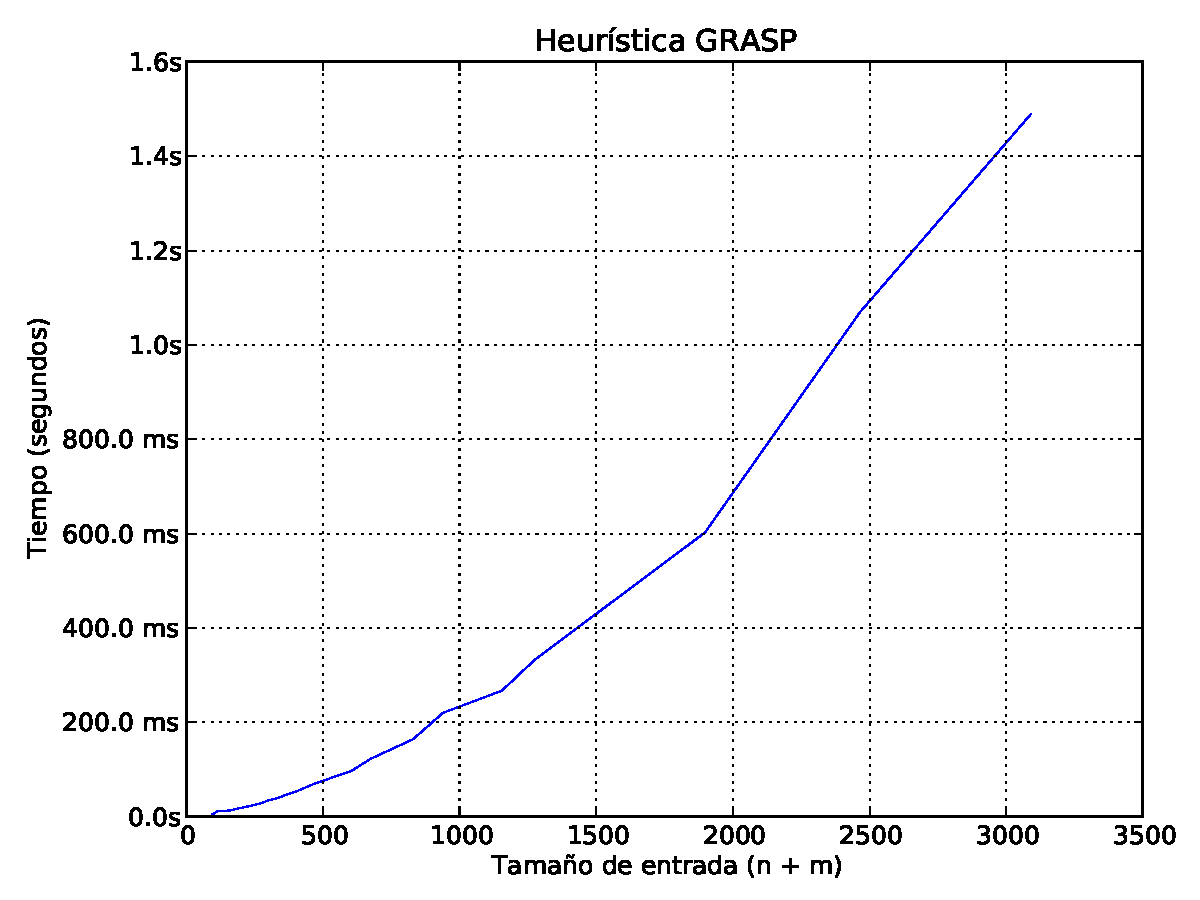
\includegraphics[angle=0, scale=.75]{imagenes/grasp_2014-06-27_19-18-59.pdf}
\label{grafico local}
\end{center}
\end{figure}

No se pareciera estar frente a una polinomio de grado 6, sin embargo, es evidente que tiene mucha más concavidad que la gráfica de la búsqueda
local. Ésto proviene trivialmente del hecho de repetir una cantidad que puede llegar a ser $n \times log(n)$ veces la búsqueda local.

Pasamos a experimentar con la calidad de la solución.

\begin{figure}[H]
\begin{center}
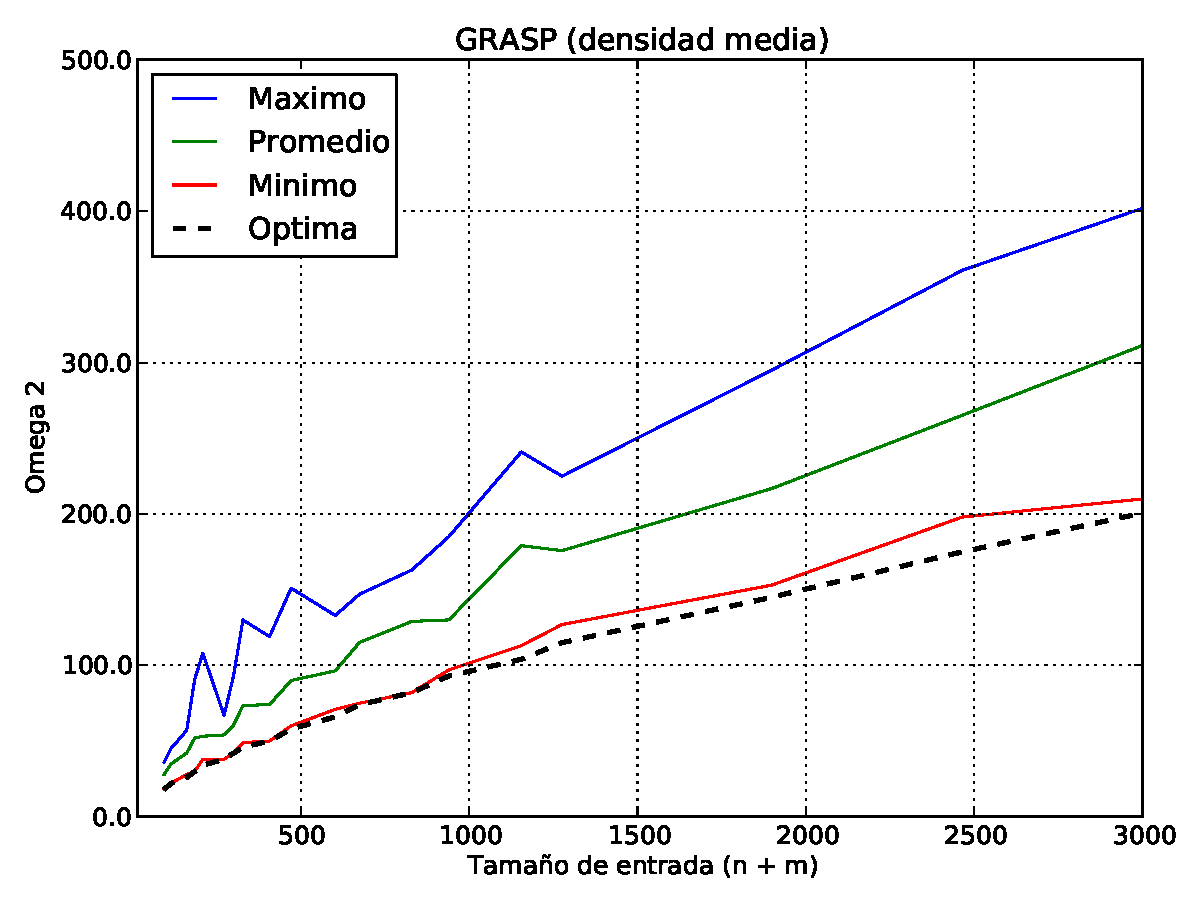
\includegraphics[angle=0, scale=.75]{imagenes/calidad_grasp_2014-06-27_08-58-53.pdf}
\label{grafico local}
\end{center}
\end{figure}

\begin{figure}[H]
\begin{center}
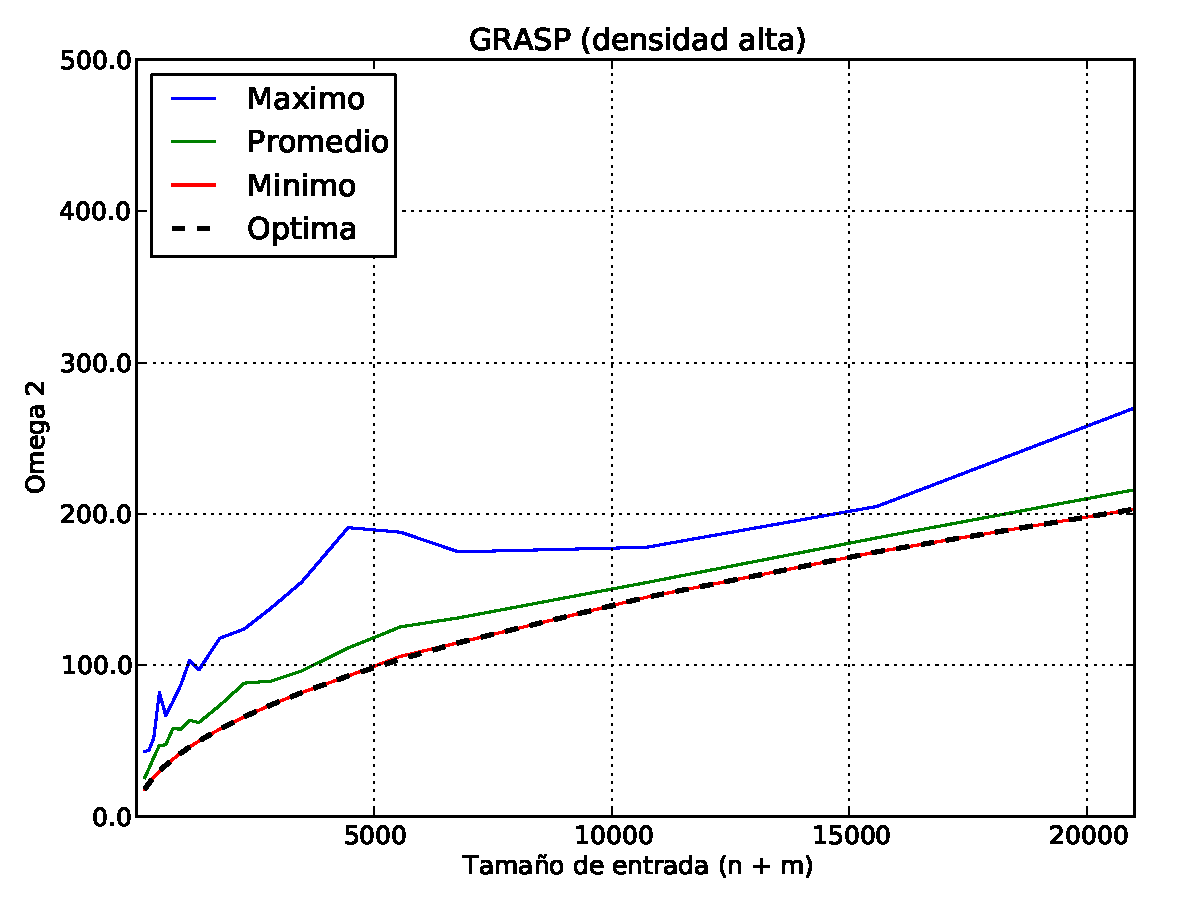
\includegraphics[angle=0, scale=.75]{imagenes/calidad_grasp_2014-06-27_08-54-46.pdf}
\label{grafico local}
\end{center}
\end{figure}

Grata fue la sorpresa al ver a GRASP en acción. Al igual que la búsqueda local, el resultado mínimo de nuestro algoritmo está muy cerca del
óptimo. Pero esta vez hemos logrado reducir la amplitud entre nuestros resultados y de esta forma acercar todo el cuerpo de nuestras soluciones
a la solución óptima.
Los buenos resultados obtenidos se deben a la naturaleza de GRASP, que consiste en iterativamente correr una búsqueda local sobre múltiples
soluciones iniciales generadas con un componente aleatorio. El repetir el experimento disminuye la varianza y garantiza una mejor solución
final.
